\documentclass[xcolor=dvipsnames,12pt]{beamer}
\usecolortheme[named=RoyalPurple]{structure}
\useoutertheme{infolines}
\usetheme{CambridgeUS}
%\usetheme[height=14mm]{Rochester}
%\hypersetup{colorlinks=true,linkcolor=yellow}
\setbeamertemplate{items}[ball]
\setbeamertemplate{blocks}[rounded][shadow=true]
\setbeamertemplate{navigation symbols}{}
\usepackage{color}
%\usefonttheme{structuresmallcapsserif}
%\usefonttheme{professionalfonts}
%\useoutertheme{default}
%\useoutertheme{infolines}


%\documentclass{beamer}
%\usecolortheme{structure}
\usepackage{graphicx}
%\usetheme{PaloAlto}
%\setbeamertemplate{items}[ball]
%\setbeamertemplate{blocks}[rounded][shadow=true]
%\useoutertheme{umbcfootline}
\newtheorem{assume}{\rlap{A}\hskip .1in}
%\newtheorem{result}{Result}[chapter]
\newcommand{\Var}  {\mbox{Var}}
\newcommand{\V} {\mbox{V}}
\newcommand{\E}  {\mbox{E}}
\newcommand{\PR}  {\mbox{P}}
\newcommand{\diag} {\operatorname*{diag}}
\newcommand{\tr} {\mbox{tr}}
\newcommand{\bmw}[1]{{\mbox{$#1$}}}
\newcommand{\MSE}{\mbox{MSE}}
\newcommand{\MSPE}{\mbox{MSPE}}


\def\bmh{{\hat \mathbf m}}
\def\bm{{\mathbf m}}
\def\bn{{\mathbf n}}
\def\mh{{\hat m}}
\def\bOmega{{\mathbf \Omega}}
\def\be{{\mathbf e}}
\def\bs{{\mathbf s}}
\def\by{{\mathbf y}}
\def\b1{{\mathbf 1}}
\def\bx{{\mathbf x}}
\def\bw{{\mathbf w}}
\def\bzero{{\mathbf 0}}

\def\bP{{\mathbf P}}
\def\bI{{\mathbf I}}
\def\bM{{\mathbf M}}
\def\bH{{\mathbf H}}
\def\bN{{\mathbf N}}
\def\bW{{\mathbf W}}
\def\bX{{\mathbf X}}
\def\bZ{{\mathbf Z}}
\def\bT{{\mathbf T}}
\def\bV{{\mathbf V}}
\def\bC{{\mathbf C}}
\def\bG{{\mathbf G}}
\def\bY{{\mathbf Y}}
\def\bD{{\mathbf D}}
\def\bS{{\mathbf S}}
\def\bR{{\mathbf R}}

\def\bbeta{\mbox{\boldmath $\beta$}}
\def\bepsilon{\mbox{\boldmath $\varepsilon$}}

% items enclosed in square brackets are optional; explanation below
\title[]{Part 1}
%\subtitle[ttt]{}
\author[Stat 801]{What is Statistics?\\
Summarizing Data}
\date{}

\begin{document}

\begin{frame}[plain]
  \titlepage
\end{frame}





\begin{frame}
\frametitle{What is statistics?}
\begin{itemize}
\item Statistics is the science of  \textcolor{magenta}{\textit{learning from data}}. 
It uses the theory of probability to make inferences about populations
or processes using data
\item For example,  we would like to know the mean  of a 
characteristic of a set of elements of a population
\item But we can't 
observe or measure each one because there are too many elements
or not all are available.
\end{itemize}
\end{frame}


\begin{frame}
\frametitle{Examples}
\begin{itemize}
\item Mean blood pressure of 40 year old pregnant females.
\item Mean lifetime of 60-watt bulbs being made at the 
G.E. plant in Cleveland.
\item Mean potency of an antibiotic after storage for 20 months on 
store shelves.
\end{itemize}
\end{frame}

\begin{frame}
\frametitle{Statistics is Useful in}
\begin{itemize}
\item Data collection
\begin{itemize}
\item Sample survey design
\item Experimental design
\end{itemize}
\item Drawing conclusion from data
\begin{itemize}
\item Descriptive methods - summarization and presentation of data
\item Statistical inference - make statements about an entire population based on a sample
\end{itemize}
\end{itemize}
\end{frame}

\begin{frame}
\frametitle{Population versus Sample}
Since we can't obtain the average exactly, we do the next best thing
\begin{itemize}
\item approximate it by finding the average for a \textcolor{magenta}{\textit{selected subset}} of 
the elements
\item we do a statistical study to estimate the population mean
\item usually, there are many objectives of a \textcolor{magenta}{\textit{statistical study}}, 
than just estimating the mean of the population.
\end{itemize}
\end{frame}


\begin{frame}
\frametitle{Steps in a Statistical Study}
\begin{itemize}
\item  \textcolor{magenta}{Collecting data} - by making observations or taking 
measurements on some sample or process of interest, possibly 
as a part of a statistically designed experiment or a survey.
\item \textcolor{magenta}{Summarizing the data}  - using statistical summary methods 
(calculating means or constructing a histogram, for example).
\item \textcolor{magenta}{Analyzing the data and making inferences} - using models
and statistical methods for drawing conclusions about the situation 
being considered.
\end{itemize}
\end{frame}


\begin{frame}
\frametitle{{Terminology and definitions}}
\begin{itemize}
\item  \textcolor{magenta}{Population} -  The set of all objects (or measurements) of 
interest; they are called elements of the population.
\item\textcolor{magenta}{Sample} - Any subset of elements from a population.

\item A statistical study is made using a sample obtained from a population.
\item Sample represents the population.
\end{itemize}
\end{frame}


\begin{frame}
\frametitle{How to Select a Sample?}
Theoretically we can get a random sample of $n$ elements by
\begin{itemize}
\item making n draws, one at a time
\item on each draw, each remaining element in the population
is \textcolor{magenta}{equally likely} to be the one drawn. 
\end{itemize}
Practically we can seldom satisfy the theoretical requirements, 
so we do the best we can to introduce randomness into our sample 
selection process. 
\end{frame}

\begin{frame}
\frametitle{How to Select a Sample? (continued)}
\begin{itemize}
\item Can the result of a statistical study of population mean
(average) be far away from the true mean?  - sure, sometimes. 
A statistical study provides evidence.  It doesn't prove anything\\
\item A random sample selected using the method described earlier 
ensures that each sample of size $n$ drawn from a population has 
the same chance of being selected
\item Methods that ensure this property are called \textcolor{magenta}{simple  random 
sampling}
\item We shall use a method for selecting a simple  random 
sample from a population in a one of our labs using random digit tables
\end{itemize}
\end{frame}


\begin{frame}
\frametitle{Some Important Definitions}
\begin{itemize}
\item  \textcolor{magenta}{Data value:} measurement
\item \textcolor{magenta}{Observation:} Row of data values
\item \textcolor{magenta}{Variable:} Set of data values for the same type of measurement
\item \textcolor{magenta}{Data set:} The entire collection of data values
\end{itemize}
\end{frame}

\begin{frame}
\frametitle{Example: Measurements on Mice}
\begin{tabular}{|c|c|c|c|}
\hline
Animal id & Cage & Weight & Length \\ \hline
1  & 1  & 22.5  & 5.3  \\ \hline
2  & 1  & 27.3  & 4.8    \\ \hline
3  & 1  & 32.2  & 4.5   \\ \hline
4  & 2  & 23.7  & 4.9  \\\hline
5 & 2  & 30.9  & 5.7   \\ \hline
6  & 2  & 22.6  &5.2   \\ \hline
\end{tabular}
\end{frame}



\begin{frame}
\frametitle{Data Description}
\begin{itemize}
\item  \textcolor{magenta}{Two broad applications of Statistics}\\[.1in]
\begin{itemize}
\item descriptive statistics
\item inferential statistics
\end{itemize}
\item When measurements from an entire population is available to us
data description will be a major objective. 
\item In this case, methods for organizing, summarizing, and describing
data are needed. 
\item  Good descriptive statistics enable us to make sense
of the data by reducing large amounts of data to a few summary
measures and graphical displays.
\end{itemize}
\end{frame}

\begin{frame}
\frametitle{Data Description - cont.}
\begin{itemize}
\item When only a random sample is available from a large population
(or a process),  inferential statistics becomes the major focus.
\item However, even in this case, descriptive statistics of the sample 
data is still important as they can be used to draw conclusions 
about the population from which the sample was taken.
\item  Data descriptions are of two types:\\[.2in]
\begin{itemize} 
\item graphical methods
\item  numerical summaries
\end{itemize}
\end{itemize}
\end{frame}


\begin{frame}
\frametitle{Graphical Methods}
\begin{itemize}
\item Bar Chart 
\item Histogram 
\item Stem-and-Leaf plot 
\item Time Series plot 
\item Boxplot 
\item Normal Probability Plot
\end{itemize}
\end{frame}


\begin{frame}
\frametitle{Numerical Summaries}
\begin{itemize}
\item Measures of Center or Location 
\begin{itemize}
\item Mode
\item Median
\item Mean 
\end{itemize}
\item Measures of Variability or Spread 
\begin{itemize}
\item Range 
\item Percentile (Quantile, Quartile)
\item Interquartile Range
\item Variance 
\item Standard Deviation
\item Coefficient of Variation 
\end{itemize}
\end{itemize}
\end{frame}


\begin{frame}
\frametitle{Histograms}
\begin{itemize}
\item To plot a histogram, a  \textcolor{magenta}{\textit{frequency table}} must first be
constructed 
\item The range of the data is divided into \textcolor{magenta}{\textit{class intervals}} or \textcolor{magenta}{\textit{bins}}
\item The number of such intervals  is determined by the
end-points of the intervals \textcolor{magenta}{\textit{number of observations}} in the data set
\item  The larger the number of observations the more the number of class intervals we may use
\item  Divide the range of data values by the  number of class intervals  to determine
an approximate \textcolor{magenta}{\textit{class width}}
\end{itemize}
\end{frame}

\begin{frame}
\frametitle{Weight gains of chicks fed an antibiotic - Data}
An animal scientist is carrying out an experiment to investigate whether adding an antibiotic to the diet of chicks will promote growth over the standard diet without the antibiotic. The scientist determines that 100 chicks will provide sufficient information to validate the results of the experiment. From previous research studies, the average weight gain of chicks fed the standard diet over an 8-week period is 3.9 grams. The scientist wants to compare the weight gain of the chicks in the study to the standard value of 3.9 grams. 
%To eliminate the effects of many other factors that could affect weight gain, the scientist rears and feeds the 100 chicks in the same building with individual feeders for each chick.
The weight gains for the 100 chicks are recorded the the table shown on the next slide.
\end{frame}


\begin{frame}
\frametitle{Example:Weight gains of chicks fed an antibiotic }
\begin{tabular}{rrrrrrrrrr}
\hline
3.7  & 4.2  & 4.4  & 4.4  & 4.3  & 4.2  & 4.4  & 4.8  & 4.9  & 4.4\\
4.2  & 3.8  & 4.2  & 4.4  & 4.6  & 3.9  & 4.1  & 4.5  & 4.8  & 3.9\\
4.7  & 4.2  & 4.2  & 4.8  & 4.5  & 3.6  & 4.1  & 4.3  & 3.9  & 4.2\\
4.0  & 4.2  & 4.0  & 4.5  & 4.4  & 4.1  & 4.0  & 4.0  & 3.8  & 4.6\\
4.9  & 3.8  & 4.3  & 4.3  & 3.9  & 3.8  & 4.7  & 3.9  & 4.0  & 4.2\\
4.3  & 4.7  & 4.1  & 4.0  & 4.6  & 4.4  & 4.6  & 4.4  & 4.9  & 4.4\\
4.0  & 3.9  & 4.5  & 4.3  & 3.8  & 4.1  & 4.3  & 4.2  & 4.5  & 4.4\\
4.2  & 4.7  & 3.8  & 4.5  & 4.0  & 4.2  & 4.1  & 4.0  & 4.7  & 4.1\\
4.7  & 4.1  & 4.8  & 4.1  & 4.3  & 4.7  & 4.2  & 4.1  & 4.4  & 4.8\\
4.1  & 4.9  & 4.3  & 4.4  & 4.4  & 4.3  & 4.6  & 4.5  & 4.6  & 4.0\\ \hline
\end{tabular}
\end{frame}


\begin{frame}
\frametitle{Creating a Histogram}
\begin{itemize}
\item It was decided to have 10 class intervals 
\item Since the range is $4.9-3.6=1.3$, a class interval width of $ 1.3/10  \approx .1 $ was used
\item The end-points of the intervals are incremented by one-half the unit of measurement (i.e., .05 gram, here)  
\item This is so that no observation falls on any
end-point
\item Since the smallest observation is 3.6 we start with the 
interval $3.55-3.65$ 
\item Once the class intervals have been determined
observations in the data set falling into each of these classes are 
tallied
\end{itemize}
\end{frame}

\begin{frame}
\frametitle{Frequency table for the chick data}
\scalebox{0.9}{
\begin{tabular}{cccc}
\hline
Class & Class Interval & Frequency $f_i$ & Relative frequency $f_i/n$\\ \hline
1 & 3.55-3.65 & 1 & 0.01\\ 
2 & 3.65-3.75 & 1 & 0.01\\ 
3 & 3.75-3.85 & 6 & 0.06\\ 
4 & 3.85-3.95 & 6 & 0.06\\ 
5 & 3.95-4.05 & 10 & 0.1\\ 
6 & 4.05-4.15 & 10 & 0.1\\ 
7 & 4.15-4.25 & 13 & 0.13\\ 
8 & 4.25-4.35 & 11 & 0.11\\ 
9 & 4.35-4.45 & 13 & 0.13\\ 
10 & 4.45-4.55 & 7 & 0.07\\ 
11 & 4.55-4.65 & 6 & 0.06\\ 
12 & 4.65-4.75 & 7 & 0.07\\ 
13 & 4.75-4.85 & 5 & 0.05\\ 
14 & 4.85-4.95 & 4 & 0.04\\ 
\textbf{Totals} & &\textbf{n=100} &\textbf{1.00}\\ \hline
\end{tabular}}
\end{frame}


\begin{frame}
\frametitle{Creating a Histogram}
\begin{center}
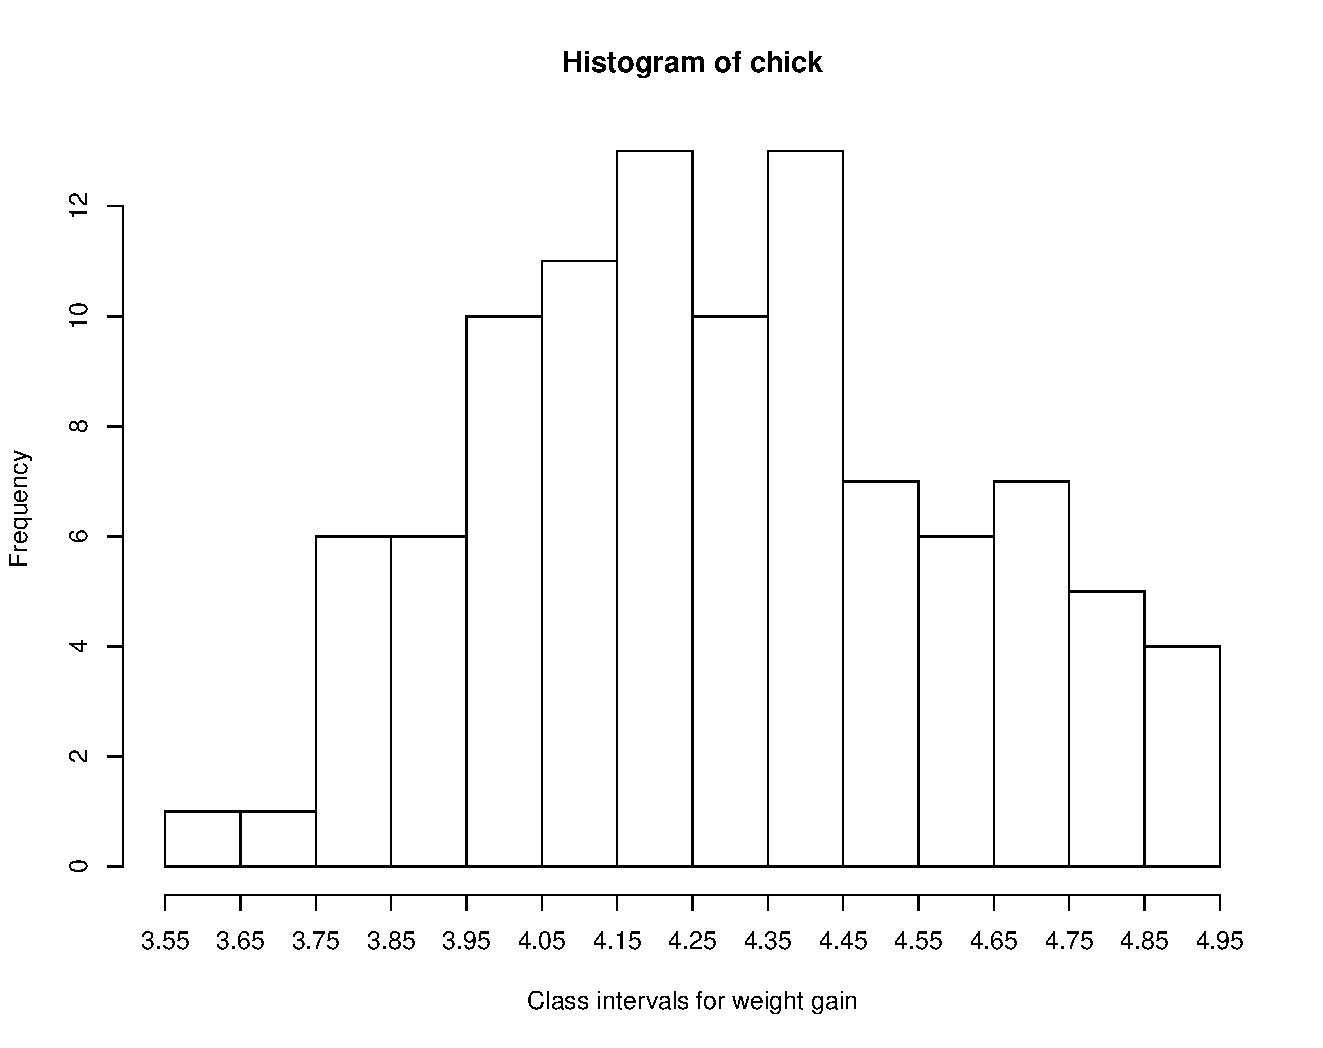
\includegraphics[scale=0.43]{chick_hist.pdf}
\end{center}
\end{frame}

\begin{frame}
\frametitle{Creating a Histogram}
Chick R code
\end{frame}

\begin{frame}
\frametitle{Stem-and-Leaf Plots}
\begin{itemize}
\item These are useful as an alternative to histograms or frequency tables.
\item The idea is to substitute digits for frequency counts used in constructing
histograms and thereby convey more information. 
\item Its profile is 
much like that of a histogram but it shows the numerical values of all
observations.
\item To construct a stem-and-leaf diagram, group each data value
into two parts:
\begin{itemize}
\item  a set of \textcolor{magenta}{leading digits}, and 
\item a set of  \textcolor{magenta}{trailing digits}.
\end{itemize} 
\end{itemize}
\end{frame}
 
\begin{frame}
\frametitle{Stem-and-Leaf Plots (continued)} 
\begin{itemize}
\item First write down, to the left of a vertical line, all possible 
values of the leading digits, in increasing order.  
\item Then we represent each data value by writing its trailing digits 
in the appropriate row to the right of the line. 
\item The column of digits on the left of the vertical
line represents the \textcolor{magenta}{stem} and the digits on the right 
the \textcolor{magenta}{leaves} of the stem-and-leaf plot.
\item Thus each data value can be 
reconstructed by combining its stem part and its leaf part. 
\item The leaves in each stem are usually written successively
(and usually contiguously) in the increasing order of magnitude. 
\end{itemize}
\end{frame}

\begin{frame}
\frametitle{Stem-and-Leaf Plots (continued)} 
In those cases where the data values may not be adequately represented by just
taking the last digits as leaves the data values must be
appropriately rounded before a stem-and-leaf diagram can be
constructed.\\
\noindent \textbf{Example}\\[.1in]
Below are the measured manganese content (in points or .01\%'s) for 20 heats of 1045 steel)
\begin{center}
\begin{tabular}{rrrrrrrr}
                             74 &  79 &  77 &  81 & 68 &  79 &  81 &  76\\
                             81 &  80 &  80 &  78 & 88 &  83 &  79 &  91\\
                             79 &  75 &  74 &  73
\end{tabular}
\end{center}
\end{frame}



\begin{frame}
\frametitle{Stem-and-Leaf Plots: Example}
A stem and leaf diagram for these data is:\\
\begin{center}
\begin{tabular}{r|l}
                                    & \\
                                  6 & 8\\
                                  7 & 344\\
                                  7 & 56789999\\
                                  8 & 001113\\
                                  8 & 8\\
                                  9 & 1
\end{tabular}
\end{center}
\end{frame}


\begin{frame}
\frametitle{Stem-and-Leaf Plots (continued)}
\begin{itemize}
\item Some sets of observations have a very narrow range that the stem and
leaf has only 2 or 3 stems.  
\item Such a plot is not useful for studying the
distribution of the data.  
\item One solution is to attempt to increase the 
number of stems, by dividing the data into subgroups within each 
original stems i.e., to use each stem value twice or more.  
\end{itemize}
\end{frame}

\begin{frame}
\frametitle{Stem-and-Leaf Plots: Example}
\begin{itemize}
\item As an example, consider the following data of height in inches
of students in a statistics class.
\item  The simplest stem-and-leaf plot is:
\begin{center}
\begin{tabular}{l|l}
                    5 & 47\\
                    6 & 02333444555556666677777889\\
                    7 & 00112223
\end{tabular}
\end{center}
\item  Obviously, this does not represent a satisfactory visual 
display of the distribution of the data.  
\end{itemize}
\end{frame}



\begin{frame}
\frametitle{Stem-and-Leaf Plots: Example}
\begin{itemize}
\item Suppose each stem is divided into two parts:
one to represent the leaves from 0 through 4 and the other for the 
leaves from 5 through 9.  
\item  The following stem-and-leaf plot is the result:
\begin{center}
\begin{tabular}{r|l}
                    5a & 4\\
                    5b & 7\\
                    6a & 02333444\\
                    6b & 555556666677777889\\
                    7a & 00112223
\end{tabular}
\end{center}
\end{itemize}
\end{frame}

\begin{frame}
\frametitle{Stem-and-Leaf Plots: Example}
\begin{itemize}
\item This may even be further improved by repeating each stem 
{\small
\begin{center}
\begin{tabular}{r|l}
                   5(01)& \\
                    (23)& \\
                    (45)& 4\\
                    (67)& 7\\
                    (89)& \\
                   6(01)& 0\\
                    (23)& 2333\\
                    (45)& 44455555\\
                    (67)& 6666677777\\
                    (89)& 889\\
                   7(01)& 0011\\
                   7(23)& 2223
\end{tabular}
\end{center}}
\end{itemize}
\end{frame}

\begin{frame}
\frametitle{Creating a Stem-and-Leaf Plot}
Stem and leaf R code
\end{frame}



\begin{frame}
\frametitle{Quantiles and Percentiles}
\begin{itemize}
\item The $80^{\rm th}$ \textcolor{magenta}{percentile} is a data value such
that approximately 80\% of the data values in the data set are 
less, and approximately 20\% are larger,  than that value.
\item  For a theoretical distribution (e.g. normal distribution) the
.8 \textcolor{magenta}{quantile}  is a value such that 80\% of the probability mass 
of the distribution lies to the left and 20\% lies to the right
of the value of the quantile.
\item  For an empirical distribution (i.e., the distribution of a data
set) we need another definition. Suppose we have  10 values in a
dataset:\ $52, 63, 67, 71, 75, 76, 76, 82, 87, 94$
\end{itemize}
\end{frame}

\begin{frame}
\frametitle{Quantiles and Percentiles}
\begin{itemize}
\item  What is the 80th percentile?  i.e., what value is such that
approximately 80\% are less and 20\% are greater? 
\item Since there are
10 values, need to find a number such that 8 values are less, 
and 2 values greater than that number.  
\item There isn't a value in the data set that satisfies both conditions. 
\item A number half way between 
82 and 87, i.e., 84.5, might be reasonably chosen as the $80^{\rm th}$
percentile.  
\item It satisfies the definition approximately.
\end{itemize}
\end{frame}

\begin{frame}
\frametitle{Quantiles and Percentiles}
\begin{itemize}
\item A definition that will give  unambiguous percentiles for any 
set of data is needed.  

\item Let $ p\ (0 < p < 100)$ denote the desired percentile,
$n$ the number of data values, and let $y_{(1)}, y_{(2)}, \ldots y_{(n)}$
denote the ordered observations so that
$$ y_{(1)} \le y_{(2)} \le \ldots  \le y_{(n)}$$
\end{itemize}
\end{frame}



\begin{frame}
\frametitle{Definition: Percentiles and Quantiles}
\begin{itemize}
\item If $p$ is one of the numbers $100(i-.5)/n$ then $y_{(i)}$ is the 
$p^{\rm th}$ \textcolor{magenta}{percentile}, for i = 1, 2, 3, ..., n-1 or n.
\item If $p$ is between $100(0.5/n)$ and $100(n-.5)/n$, and $p$ is not
one of the numbers $100(i-.5)/n$ then the percentile is obtained 
by linear interpolation between the two percentiles that bracket $p$.
\item {\tt Quantiles} are a generalization of percentiles. The 
$p^{\rm th}$ quantile of a dataset is the $100p^{\rm th}$
percentile. 
\end{itemize}
\end{frame}

\begin{frame}
\frametitle{Quantiles and Percentiles}
Thus the  $p^{\rm th}$  \textcolor{magenta}{quantile} 
of the  dataset $y_{(1)}, y_{(2)}, \ldots y_{(n)}$ is obtained as follows:
\begin{enumerate}
\item If $p$ is one of the numbers $(i-.5)/n$ then $y_{(i)}$ is the 
$p^{\rm th}$ quantile, for i = 1, 2, 3, ..., n-1 or n.
\item  If $p$ is between $(0.5/n)$ and $(n-.5)/n$, and $p$ is not
one of the numbers $(i-.5)/n$ then the quantile is obtained 
by linear interpolation between the two quantiles that bracket p.
\item The $p_i^{\rm th}$ quantile of a dataset is denoted by $Q(p_i)$
\end{enumerate}
\end{frame}


\begin{frame}
\frametitle{Quantiles and Percentiles: Example}
Suppose we have a dataset consisting of the 10 observations:
$9.614,  9.614,  10.688,  7.583,  8.572,  8.527,  8.577,  9.471,
9.165,  9.011$ The following table shows the ordered data values as
the specified \textcolor{magenta}{quantiles}:
{\footnotesize
\begin{center}
\begin{tabular}{|c|c|c|} \hline
 \multicolumn{1}{|c|}{$i$} &\multicolumn{1}{c|}{$p_i=(i-.5)/10$} &
\multicolumn{1}{c|}{$Q(p_i)$} 
                 \\ \hline
 1 & 0.05 & 7.583\\
 2 & 0.15&   8.527\\
 3 & 0.25 &  8.572 \\
 4 & 0.35 &  8.577  \\
 5 & 0.45 &  9.011\\
 6 & 0.55 &  9.165\\
 7 & 0.65 &   9.471 \\
 8 & 0.75 &    9.614 \\
 9 & 0.85 &  9.614  \\ 
 10 & 0.95 &  10.688\\ \hline
\end{tabular}
\end{center}}
\end{frame}



\begin{frame}
\frametitle{Quantiles by Linear Interpolation}
\begin{itemize}
\item $Q(p)$ for values of $p = (i-.5)/n$ correspond to
the ordered observations for $i = 1, 2, \ldots, n$. For example 
$Q(.55)=9.165$. 
\item How is, say, $Q(.525)$ determined? This is obtained by
linear interpolation between the two quantiles that bracket $.525$
i.e, $Q(.45)$ and $Q(.55)$.
\item For a $p$ such that $p_i < p < p_{i+1},\ Q(p)$ is computed as 
the weighted average $Q(p) = (1-f)Q(p_i) + fQ(p_{i+1})$ where 
$f =(p-p_i)/(p_{i+1}-p_i) = n(p-p_i)$
\end{itemize}
\end{frame}

\begin{frame}
\frametitle{Quantiles by Linear Interpolation: Example}
\begin{itemize}
\item Suppose $n = 10$ and one needs to compute  $Q(.525)$.  
\item Since  
$.45 < p < .55, \ f = 10 (.525 - .45)  = .75$. 
\item Thus  $Q(.525)=.25Q(.45) +
.75Q(.55)$.
\item In the above example, therefore $$Q(.525)= .25(9.011)+.75(9.165)=9.1265$$
\end{itemize}
\end{frame}


\begin{frame}
\frametitle{Box Plots (Tukey, 1977)}
The  boxplot is a summary display of a set of data, that is useful for
studying the shape of the distribution including its
symmetry or asymmetry  around the central location, based on the quantiles
$Q_1,\ M$, and $Q_3$ as defined below:
\begin{itemize}
\item Upper Quartile = $75^{ th} { percentile} =Q(.75)=Q_3$
\item Median  = $50^{ th} { percentile} =Q(.50)=M$
\item Lower Quartile  = $25^{ th} {percentile} =Q(.25)= Q_1$
\item Interquartile Range (IQR) = \\
 Upper Quartile -  Lower Quartile  =$Q_3- Q_1$
\end{itemize}
\end{frame}



\begin{frame}
\frametitle{Box Plots (continued)}
 The following quantities also need to be
computed for constructing a box plot:
\begin{itemize}
\item Upper Fence =  $Q_3 + 1.5$ IQR. 
\item Lower Fence =  $Q_1 - 1.5$ IQR.
\item Upper Adjacent Value:  the largest observation  below the upper fence
\item Lower Adjacent Value:  the smallest observation above the lower fence   
\item Outside Values:  Observations that fall outside adjacent values.  
\end{itemize}
\end{frame}



\begin{frame}
\frametitle{Box Plots: Example}
\scalebox{0.6}{
\begin{picture}(200,290)(-90,20)
\setlength{\unitlength}{.35mm}
\put(60,100){\framebox(20,140){}}
\put(60,140){\line(1,0){20}}
\put(70,240){\line(0,1){60}}
\put(70,60){\line(0,1){40}}
\put(85,240){\small $Q_3$ (.75 Quantile)}
\put(85,140){\small Median(.5 Quantile)}
\put(85,100){\small $Q_1$ (.25 Quantile)}
\put(85,290){\small Upper Adjacent Value}
\put(85,315){\small Outside Values}
\put(70,305){*} 
\put(70,315){*}
\put(85,60){\small Lower Adjacent Value}
\end{picture}}
\end{frame}


\begin{frame}
\frametitle{Creating a Stem-and-Leaf Plot}
boxplot R code
\end{frame}




\begin{frame}
\frametitle{Side-by-side box plots}
\begin{itemize}
\item Useful comparing distributions of variables across subsamples 
defined by values of a categorical variable. 
\item Example 
\begin{itemize}
\item Side-by-side box plots for an epilepsy study
\item 59 patients
\item The patients were randomly assigned to receive the
anti-epileptic drug \textcolor{magenta}{Progabide} or a \textcolor{magenta}{placebo}. 
\item The side-by-side boxplots of  \textcolor{magenta}{baseline seizure rates} for 
each of the two groups are shown below
\end{itemize}
\end{itemize}
\end{frame}


\begin{frame}
\frametitle{Side-by-side box plots of epilepsy data}
\begin{center}
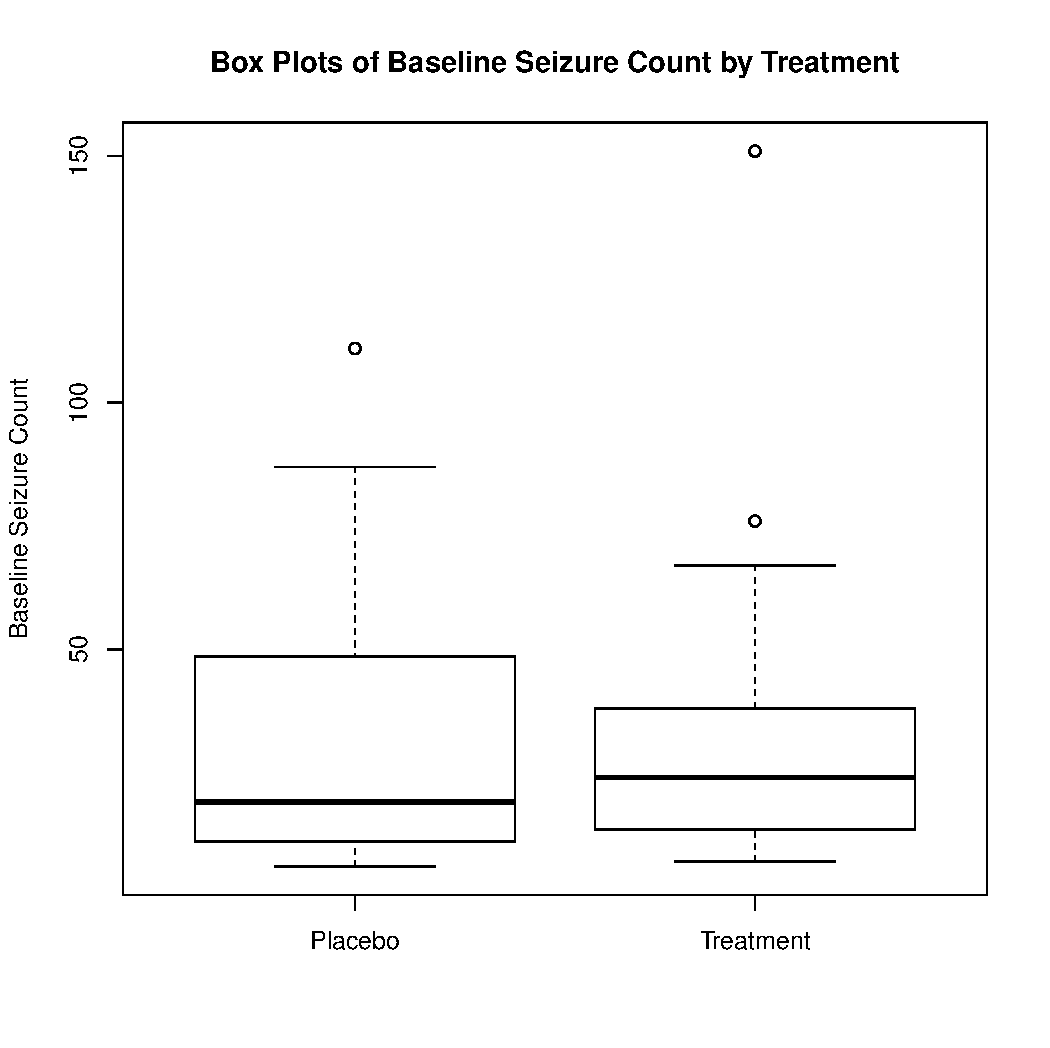
\includegraphics[scale=0.43]{epilepsy_boxplot.pdf}
\end{center}
\end{frame}



\begin{frame}
\frametitle{Normal Probability Plot}
\begin{itemize}
\item Consider a sample $y_1, y_2, \ldots, y_n$ of size $n$.  
\item The data are first ordered in increasing order of magnitude.
\item Then a value
$p$ is assigned to each data value using the formula $p = (i -
0.5)/n$.
\item Thus the ordered data values will be the $p_i^{\rm th}$
quantile $Q(p_i)$  for $i=1,2,\ldots,n.$
\item Example: Quantiles for a data set with $n = 18$
\end{itemize}
\end{frame}

\begin{frame}
\frametitle{Summation Notation}
http://www.columbia.edu/itc/sipa/math/summation.html
\end{frame}

\begin{frame}
\frametitle{Quantiles}
\begin{center}
\scalebox{0.75}{
\begin{tabular}{@{\extracolsep{.2in}}r|r|c|r} 
\hline
$i$ & \multicolumn{1}{c|}{$y_i$} &
    \multicolumn{1}{c|}{$p_i = (i - 0.5)/18$} &
    \multicolumn{1}{c}{$z_p$} \\ \hline
1 & 57 & 1/36 = 0.0278 & -1.9145 \\
2 & 58 & 3/36 = 0.0833 & -1.3830 \\
3 & 59 & 5/36 = 0.1389 & -1.0853 \\
4 & 59 & 7/36 = 0.1944 & -0.8616 \\
5 & 59 & 9/36 = 0.2500 & -0.6745 \\
6 & 60 & 11/36 = 0.3055 & -0.5085 \\
7 & 61 & 13/36 = 0.3611 & -0.3555 \\
8 & 62 & 15/36 = 0.4167 & -0.2104 \\
9 & 62 & 17/36 = 0.4722 & -0.06968 \\
10 & 62 & 19/36 = 0.5278 & 0.06968 \\
11 & 63 & 21/36 = 0.5833 & 0.2104 \\
12 & 63 & 23/36 = 0.6389 & 0.3555 \\
13 & 63 & 25/36 = 0.6944 & 0.5085 \\
14 & 64 & 27/36 = 0.7500 & 0.6745 \\
15 & 64 & 29/36 = 0.8056 & 0.8616 \\
16 & 65 & 31/36 = 0.8611 & 1.0853 \\
17 & 67 & 33/36 = 0.9167 & 1.3830 \\
18 & 69 & 35/36 = 0.9722 & 1.9145 \\ \hline
\end{tabular}}
\end{center}
\end{frame}


\begin{frame}
\frametitle{Normal Probability Plot:Example}
\begin{itemize}
\item The quantile of the standard normal distribution, $z_p$,
corresponding to each $p$ value, is then computed using
the table of Normal percentiles (i.e. the $z$-table).
\item
The Normal Probability plot is the plot of the quantiles $Q(p)$
of the data vs. $z_p$, the corresponding standard normal quantiles. 
\item
Thus this plot is also called the quantile-quantile plot or the 
Q-Q plot, in general.
\end{itemize}
\end{frame}


\begin{frame}
\frametitle{Normal Probability Plot: Example}
\begin{center}
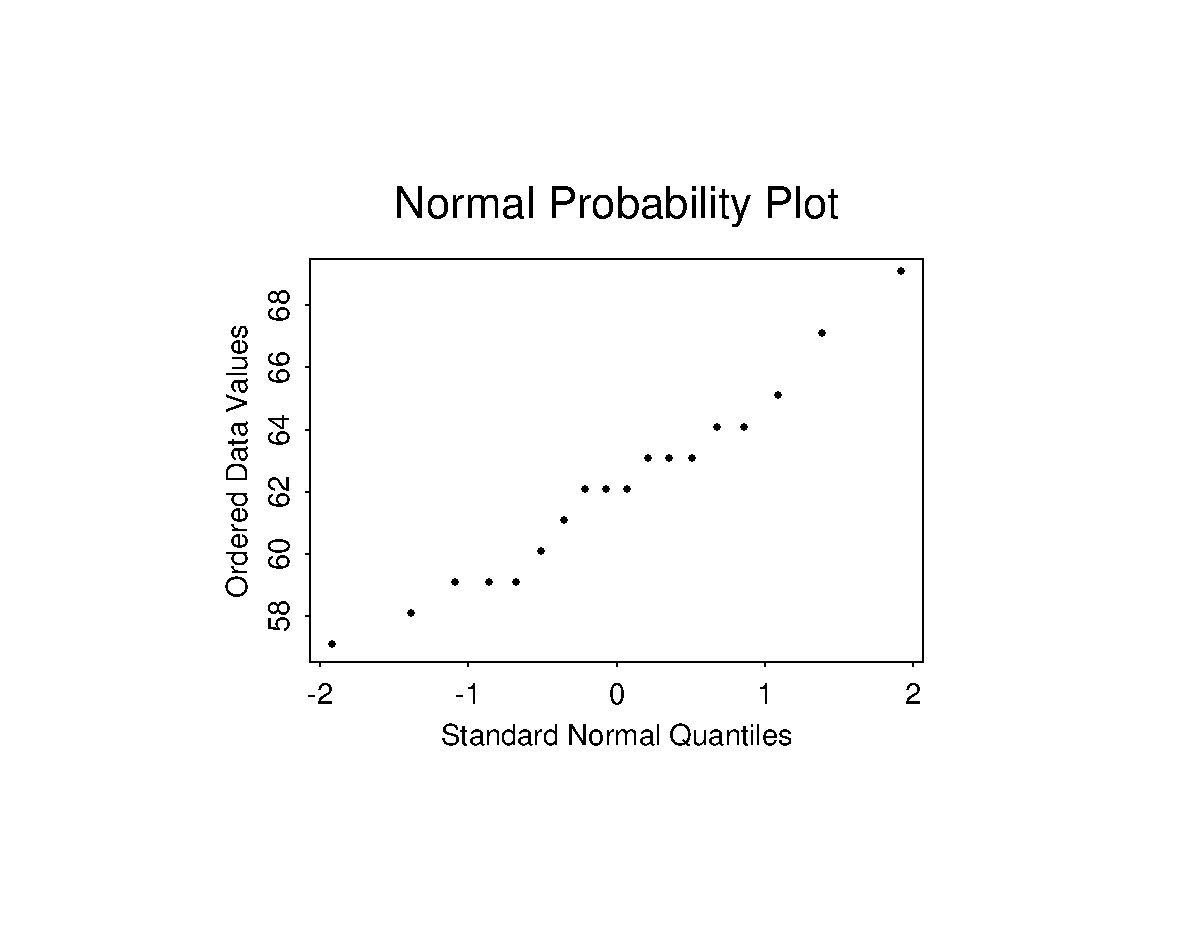
\includegraphics[scale=0.5]{normplot.pdf}
\end{center}
\end{frame}


\begin{frame}
\frametitle{Normal Probability Plot (continued)}
\begin{itemize}
\item If the data is a random sample from a normal population  
the plotted points will lie approximately in a \textcolor{magenta}{straight-line}.
\item \textcolor{magenta}{Departures} from a straight-line may indicate that the population
distribution is different from a Normal distribution.  
\item Specific types of departures can be used to identify how the population
distribution differs from a Normal distribution.
\item The following pages contains  normal robability plots of
computer generated data from populations that resemble distributions
that are as described. 
\end{itemize}
\end{frame}


\begin{frame}
\frametitle{Normal Probability Plot (continued)}
\begin{center}
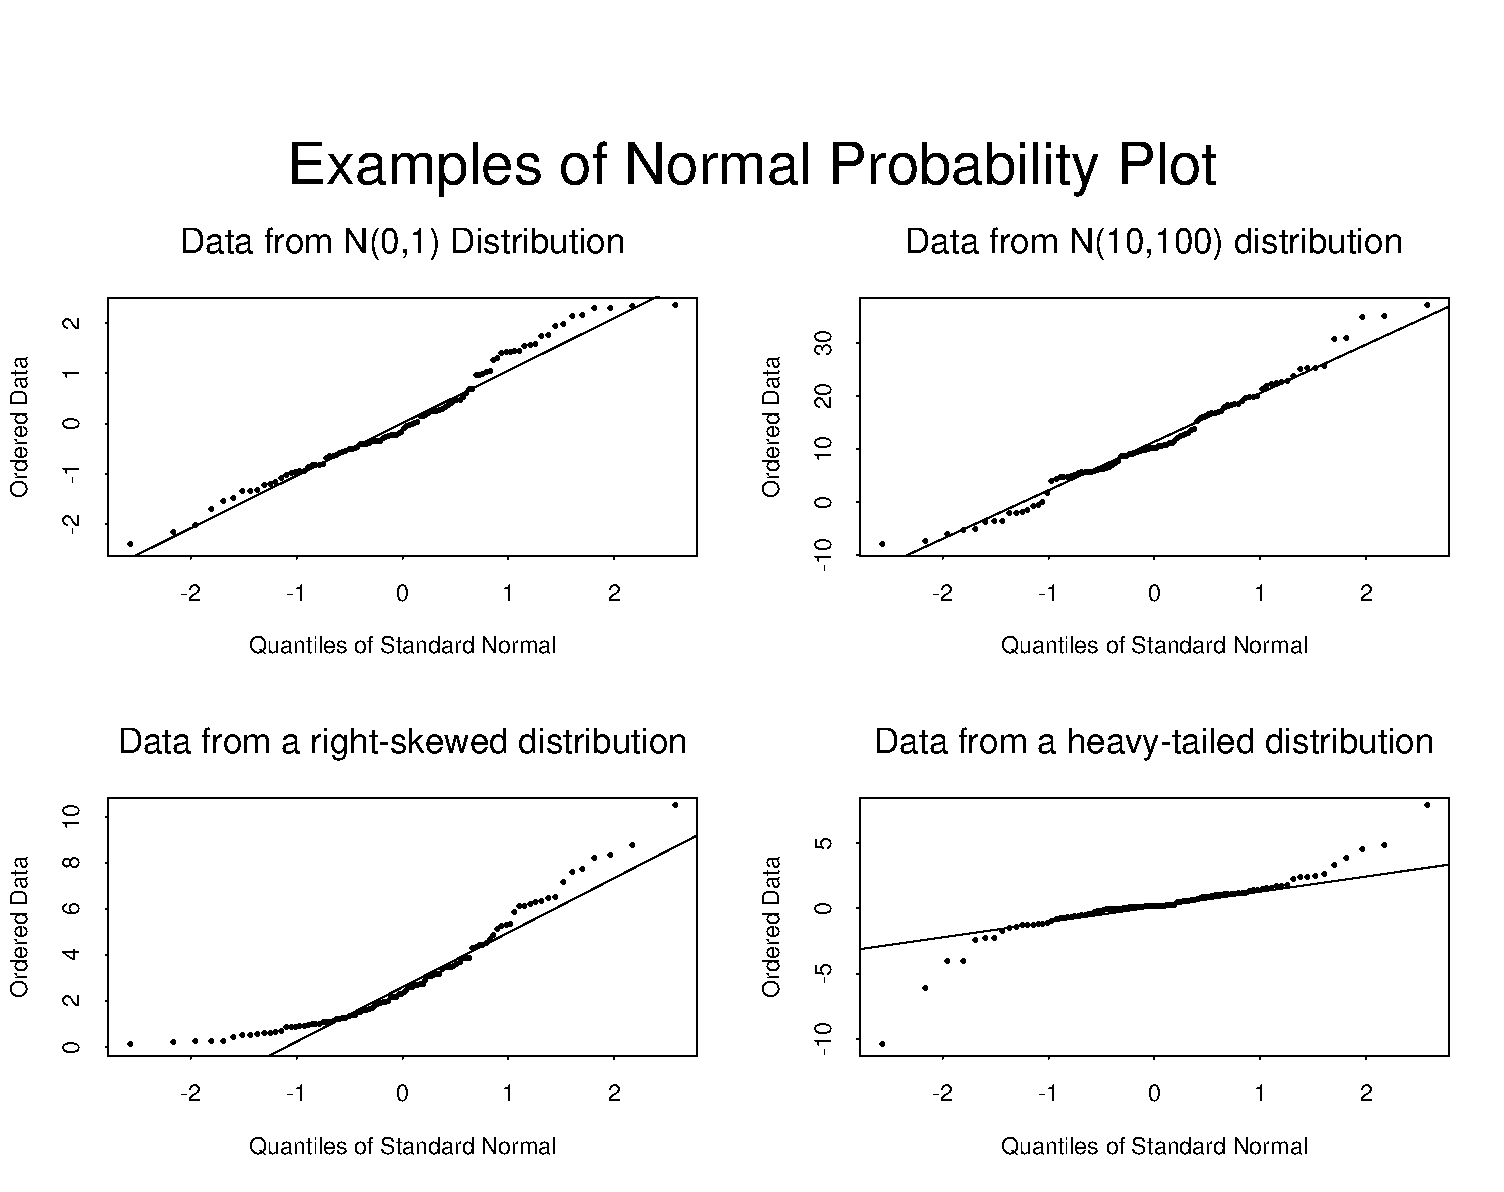
\includegraphics[scale=0.35]{normplot2.pdf}
\end{center}
\end{frame}

\begin{frame}
\frametitle{Normal Probability Plot (continued)}
\begin{itemize}
\item The top set of plots are from normal populations
with different mean and variance parameters
\item The bottom two 
are from populations that differ in shape from the normal distribution. 
\item Notice that the bottom two plots show specific patterns (the left
graph shows a bowl-shape while the other shows an inverted S-shaped
pattern). 
\item These are markedly different from the deviation from a
straight line shown in the top graphs which are only due to random
variation.
\end{itemize}
\end{frame}

%----------------------------------------------------------------

\begin{frame}
\frametitle{Sample Statistics vs. Parameters}
\begin{itemize}
\item A \textcolor{magenta}{parameter} is a descriptive statistic of a population.
\item A \textcolor{magenta}{sample statistic} is a descriptive statistic of a
sample.
\item Take a \textcolor{magenta}{census} of a population recording values of
 a variable as $x_1, x_2,\ldots,x_N$, where $N$ is the population
size, then
\begin{itemize}
\item Population mean, $\mu=\frac{\textstyle\sum x}{N}$
\item Population variance, $\sigma^2=\frac{\textstyle\sum (x-\mu)^2}{N}$
\item Population standard deviation, $\sigma=\sqrt{\sigma^2}$
\end{itemize}
\end{itemize}
\end{frame}


\begin{frame}
\frametitle{Sample Statistics vs. Parameters}
\begin{itemize}
\item Since censuses cannot be taken for every population we wish to study, 
parameters  cannot be exactly calculated and thus are usually
unknown.
\item Instead, a \textcolor{magenta}{random sample} of a population is taken recording  values of
a variable as $x_1, x_2,\ldots,x_n$, where $n$ is the sample
size, then
\begin{itemize}
\item sample mean (average, arithmetic mean), $\bar{x}= \frac{\textstyle \sum x}{n}$
\item  sample variance, $s^2=\frac{\textstyle \sum (x-\bar{x})^2}{n-1}$
\item sample standard deviation, $s=\sqrt{s^2}$
\end{itemize}
\end{itemize}
\end{frame}


\begin{frame}
\frametitle{Sample Statistics vs. Parameters}
\begin{itemize}
\item $\mu$, $\sigma^2$, and $\sigma$ are \textcolor{magenta}{parameters}.
\item $\bar{x}$, $s^2$, and $s$ are \textcolor{magenta}{sample statistics}.
\end{itemize}
\end{frame}


%----------------------------------------------------------------
\begin{frame}
\frametitle{Sample Statistics vs. Parameters: Example}
Calculate the sample mean, variance, and standard deviation for data: 2, 3, 3, 4, 3.
\begin{center}
\begin{tabular}{@{\extracolsep{.15in}}lrr}
\hline
$i$ & $x$ & $x^2$ \\ \hline
1 & 2 & 4\\
2 & 3 & 9\\
3 & 3 & 9\\
4 & 4 & 16\\
5 & 3 & 9 \\ \hline
 & $\sum x=15$ & $\sum x^2= 47$ \\ \hline
\end{tabular}
\end{center}
\end{frame}

\begin{frame}
\frametitle{Sample Statistics vs. Parameters}
Compute sample variance $s^2$ and sample standard deviation
$s$.
\begin{eqnarray*}
s^2 & = &\frac{\textstyle\sum x^2 - \frac{(\textstyle\sum
x)^2}{n}}{n-1}=\frac{47-\frac{(15)^2}{5}}{5-1}=2/4=0.5\\[.1in]
 s & = & \sqrt{(s^2)}=\sqrt{0.5}=0.71
\end{eqnarray*}
\end{frame}


\begin{frame}
\frametitle{Problems with the Variance and Standard Deviation}
\begin{itemize}
\item The units of the variance are squared
\item The standard deviation has the same units as the data
\item Both $s$ and $s^2$ are absolute measures of variation, and many times the $s$ and $s^2$ cannot be compared for two different variables
\end{itemize}
\end{frame}

\begin{frame}
\frametitle{Problems with the Variance and Standard Deviation - Example}
\begin{itemize}
\item We would like to compare the standard deviation of auto speeds on I-80 with the German Autobahn, but speeds on I-80 are in MPH while speeds on the Autobahn are in km per hour.
\end{itemize}
\begin{center}
\begin{tabular}{@{\extracolsep{.15in}}l|cc}
\hline
 & I-80 & Autobahn \\ \hline
$s^2$ & 144 & 625\\
$\bar{x}$ & 63 & 120 \\ \hline
\end{tabular}
\end{center}
\end{frame}

\begin{frame}
\frametitle{Coefficient of Variation}
\begin{itemize}
\item It is a relative measure of variability.
\item  \textcolor{magenta}{Coefficient of Variation:} $\frac{s}{\bar{x}}\times 100$ 
\end{itemize}
\end{frame}

\begin{frame}
\frametitle{Coefficient of Variation - Example}
\begin{center}
\begin{tabular}{@{\extracolsep{.15in}}l|cc}
\hline
 & I-80 & Autobahn \\ \hline
$s^2$ & 144 & 625\\
$\bar{x}$ & 63 & 120 \\ \hline
$\frac{s}{\bar{x}}\times 100$ & $19\%$ & $20\%$ \\ \hline
\end{tabular}
\end{center}
\end{frame}

\begin{frame}
\frametitle{Numerical Summary Measures}
\begin{itemize}
\item The sample mean and the sample median are examples of  \textcolor{magenta}{numerical
descriptive measures} of the  \textcolor{magenta}{central tendency} of a
sample and describes the center or location around which the data 
are distributed.
\item   The sample variance and standard deviation are  
examples of \textcolor{magenta}{numerical descriptive measures} of the 
 \textcolor{magenta}{variability} or the  \textcolor{magenta}{spread} of the sample around the center.
\item These  numerical descriptive measures are used both to describe 
a population, if the entire  population of measurements is available,
(e.g., census) or,
 to draw inferences about a population
from the statistics calculated on  a random sample drawn 
from the  population.
\end{itemize}
\end{frame}

\begin{frame}
\frametitle{Other Numerical Summary Measures - Median}
\textcolor{magenta}{Median:} Value at which $50\%$ of the observations are above and $50\%$ below.\\
Computation of the sample median from a sample of size n:
\begin{itemize}
\item Arrange observations in ascending order
\item The value of the $\left(\frac{n+1}{2}\right)^{th}$ ordered observation is the median
\end{itemize}
 What is the median of $2,4,6,8,10$?\\
 What is the median of $2,4,6,10$?\\
 Location or spread?
\end{frame}

\begin{frame}
\frametitle{Other Numerical Summary Measures - Mode}
\textcolor{magenta}{Mode:} Value which appears the most frequently.\\
What is the mode?
\begin{itemize}
\item We count beetles on 12 plants, and 6 of them do not have any, but the other 6 has $3,2,6,1,5,6$.
\item We count beetles on 12 plants, and 4 of them do not have any, 4 of them have 2 and 4 of them have 5.
\end{itemize}
Location or spread?
\end{frame}

\begin{frame}
\frametitle{Which measure of location should be used?}
\begin{itemize}
\item When the data are symmetric?
\item When data are skewed? Which means that there are some very large or very small values?
\end{itemize}
\end{frame}

\begin{frame}
\frametitle{Example - Which measure of location should be used?}
Skewed distribution R code
\end{frame}

\begin{frame}
\frametitle{Estimate of the Standard Error of the Sample Mean}
$\frac{s}{\sqrt{n}}$
\end{frame}

\end{document}






 

 

 
